\documentclass[12pt]{article}

\usepackage[hidelinks]{hyperref}
\usepackage{graphicx}
\usepackage{color}
\usepackage{xcolor}
\usepackage{listings}
\usepackage{courier}
\usepackage{amsmath}

% syntax highlighting from: http://www.kv0.org/blog/2010/12/15/vernunftiges-syntax-highlighting-in-latex/
\lstset{
	basicstyle=\footnotesize\ttfamily, % Standardschrift
	numbers=left, % Ort der Zeilennummern
	numberstyle=\tiny, % Stil der Zeilennummern
	%stepnumber=2, % Abstand zwischen den Zeilennummern
	numbersep=5pt, % Abstand der Nummern zum Text
	tabsize=2, % Groesse von Tabs
	extendedchars=true, %
	breaklines=true, % Zeilen werden Umgebrochen
	keywordstyle=\color{orange}\bfseries,
	frame=b,
	% keywordstyle=[1]\textbf, % Stil der Keywords
	% keywordstyle=[2]\textbf, %
	% keywordstyle=[3]\textbf, %
	% keywordstyle=[4]\textbf, \sqrt{\sqrt{}} %
	stringstyle=\color{white}\ttfamily, % Farbe der String
	showspaces=false, % Leerzeichen anzeigen ?
	showtabs=false, % Tabs anzeigen ?
	xleftmargin=17pt,
	framexleftmargin=17pt,
	framexrightmargin=5pt,
	framexbottommargin=4pt,
	commentstyle=\color{green},
	% backgroundcolor=\color{gray},
	showstringspaces=false, % Leerzeichen in Strings anzeigen ?
	morekeywords={__global__} % CUDA specific keywords
}
\lstloadlanguages{% Check Dokumentation for further languages ...
%[Visual]Basic
%Pascal
C,
C++,
%XML
%HTML
Java
}
%\DeclareCaptionFont{blue}{\color{blue}}
 
%\captionsetup[lstlisting]{singlelinecheck=false, labelfont={blue}, textfont={blue}}
\usepackage{caption}
\DeclareCaptionFont{white}{\color{white}}
\DeclareCaptionFormat{listing}{\colorbox{gray}{\parbox{\textwidth}{\hspace{15pt}#1#2#3}}}
\captionsetup[lstlisting]{format=listing,labelfont=white,textfont=white, singlelinecheck=false, margin=0pt, font={bf,footnotesize}}

\title{Project Report - First assignment - GAME ENGINES}
\author{Andrea Distler}
\date{28 November, 2012}

\begin{document}
\maketitle
\newpage

\tableofcontents
\newpage

%------------------------------------------
\section{Introduction}
This is the project report for the first assignment of the Game Engines course.

A short description of the source code and the used libraries can be found in section \ref{section:files}. The files are available on GitHub. The libraries are also made available on GitHub for easier installation.

Section \ref{section:outcome} describes the outcome of the project. 

Section\ref{section:overview} gives an overview of the used mechanics and points out the key features of the project. 

Section \ref{section:classes} gives a detailed description of the important classes and their relations to each other. It also points out challenging parts of the code.

I have invested an unnecessarily big amount of time into this small assignment, and I want to elaborate on my workflow in section \ref{section:workflow}.

%------------------------------------------
\section{The Files}
\label{section:files}
All files can be found on GitHub. \newline 
\url{https://github.com/JungleJinn/GE---SimplePlatformerEngine}.

\subsection{Used Libraries}

The project was written in C++, using additional libraries:

\begin{itemize}
\item{
	Included in the repository
	\begin{itemize}
		\item{SDL image}
	\end{itemize}
}

\item{
	External
	\begin{itemize}
		\item{openGL. Installed manually. Files in zip}
		\item{glm. Installed manually. Files in zip}
		\item{SDL 1.2.15. \url{http://www.libsdl.org/download-1.2.php} Used environment variable named SDK\_SDL}
	\end{itemize}
}
\end{itemize}

%------------------------------------------
\section{Outcome}
\label{section:outcome}

The project's result is a little game in which the player can control a bomb. The player cannot directly control the bomb's position. However, it is possible to change the bomb's mass and therefore indirectly possible to steer the bomb. The goal of the game is to survive as long as possible, which is made hard by other bombs which present themselves as obstacles. Depending on the player's mass, the enemy bomb will affect the player's further movement. If the player moves backwards, the game is over. For a screenshot of the game see figure \ref{figure:outcome}.

There is a short explanation of the controls and rules of the game in the beginning. Once a player loses, there is also a gameover screen, telling the player that the game is now over.

The assignment was to create a simple physics engine which can be used for a platformer. The game features:

\begin{itemize}
	\item{2D physics}
	\item{openGL rendering}
	\item{an intro screen and an outro screen}
	\item{a dragon with a hat}
	\item{sprites and texture atlases}
	\item{collision detection and response}
	\item{bounciness}
	\item{very intuitive controls}
\end{itemize}

\begin{figure}[H]
	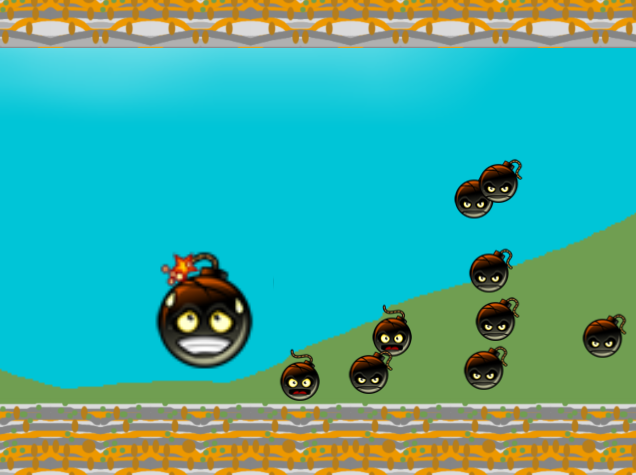
\includegraphics[width=\textwidth]{outcome.png}
	\caption{A screenshot of the game.}
	\label{figure:outcome}
\end{figure}

% -----------------------------------------
\newpage
\section{Overview}
\label{section:overview}

This section gives an overview over used mechanics.

\subsection{Game Loop}

\begin{lstlisting}[caption=The game loop, language=C++]
lastUpdateTime = clock();
Init();

quit = false;
while (!quit)
{
	Play();
}
\end{lstlisting}

First the game is being set up, then the game loop starts. The game loop is quite basic. While the game has not been quit, it is playing.\newline

\subsection{Messaging}

The Input is realized by using SDL events. The first thing done in the Play method is to fetch all pending input events. These events are then sorted by what is important, what is to be used in the game, and what not. Then the newly written message system starts to create and forward messages.

The messenger can send messages of different types to receivers of type IMessageReceiver. All objects of this type automatically register and unregister at the messenger at creation and deletion. The receivers decide which kinds of messages they want to process, but each receiver gets all sent messages.

\begin{lstlisting}[caption=Messaging, language=C++]
SDL_Event sdlEvent = SDL_Event();
while (SDL_PollEvent(&sdlEvent))
{
	// user closes window
	if (sdlEvent.type == SDL_QUIT)
	{
		quit = true;
		break;
	}
	else if (sdlEvent.type == SDL_KEYDOWN)
	{
		messenger->SendMessage(InputMessage(InputMessage::KEY_DOWN, sdlEvent.key.keysym.sym));
	}
	else if (sdlEvent.type == SDL_KEYUP)
	{
		messenger->SendMessage(InputMessage(InputMessage::KEY_UP, sdlEvent.key.keysym.sym));
	}
}
\end{lstlisting}

\subsection{Physics}

The physics are calculated in two dimensions. The physics system is responsible for movement and for collisions as well as for collision response. Bodies are implemented as simple rigid bodies. Forces can be applied. There are two basic collision shapes: Circles and Rectangles. The collision detection happens in two states, first the broad phase, which only checks the radius of the objects, and the narrow phase, in which the collision normal is calculated. The normal is then used to determine the resulting forces acting on both colliders. Bodies have a coefficient of restitution which adds to the collision response. The combination method is to use the average coefficient of restitution of both bodies.

For integrating forces, the integration method receives a value named deltaTime. The delta time is calculated like in the following listing:

\begin{lstlisting}[caption=deltaTime, language=C++]
int now = clock();
deltaTime = (float)((now - lastUpdateTime) / CLOCKS_PER_SEC) / timeScale;
lastUpdateTime = now;
\end{lstlisting}

The whole game execution can be slowed or fastened by setting different timeScale values. At a value of 1.0 it is executed in real-time, and other values stretch or squish the perceived time.

\subsection{Sprites}

Sprites are used for the player and for the enemy bombs. They are stored in a spritesheet and their texture coordinates are adapted to fit certain sprite frames.

\subsection{Camera}

The camera is moving with the player all the time. A problem encountered with a potentially endless level was whether the floor and ceiling should always be recreated. The player can move as far as he wants to, therefore an inifinite amount of rectangular walls would be needed. The solution which avoids creating endless amounts of floor tiles was to always move the floor and ceiling with the player (not unlike the camera). The texture coordinates change to create the visual feedback of the player's velocity. The illusion that the player moves in relation to the floor is created, whereas the player and the floor have a relative velocity of zero. The background also follows the player.

\subsection{Dragon}

In the first phase of the game the player can choose the launch angle by rotating a dragon's head.

%-----------------------------------------
\section{Important Classes}
\label{section:classes}

In figure \ref{figure:classes} a selection of classes is depicted. The most interesting parts are described in this chapter.

\subsection{Game}
\label{subsection:Game}
The game class manages the game states and the game objects. It renders the objects and updates them automatically. The game class is intended to serve as a base class for other games, although it was used as both the abstract class and the implementation in this project.

\paragraph{Initialization.} First of all, SDL is set up. After that, openGL is prepared for 2D drawing. The projection mode used is orthogonal.
After the graphics setup, the frame for the game logic is initialized. This includes the messenger (\ref{subsection:Messenger}), the log, and the physics (\ref{subsection:Physics}).
Subsequently the game objects are set up. \texttt{GameObjects} need a reference to the game and the messenger, which they use for automatically registering. \texttt{GameObject}s in this game are the playerBomb, floor, ceiling, dragon, and the background. The enemy bombs are spawned at run-time.

\paragraph{Play.} First, all relevant events from SDL are converted to \texttt{Message}s and broadcast by the messenger. Then \texttt{deltaTime} is calculated. The game, physics and gameObjects are updated after. The render method is called afterwards. When the game objects are updated, the game loops through the list containing them. If a game object has to be deleted it cannot be done in this loop, so the object is moved to a deletion list. Deleting gameObjects is the last thing to do in the \texttt{Play} method.

\begin{lstlisting}[caption=The play method.,language=C++]
void Game::Play()
{
	// events
	SDL_Event sdlEvent = SDL_Event();
	while (SDL_PollEvent(&sdlEvent))
	{
		// user closes window
		if (sdlEvent.type == SDL_QUIT)
		{
			quit = true;
			break;
		}
		else if (sdlEvent.type == SDL_KEYDOWN)
		{
			messenger->SendMessage(InputMessage(InputMessage::KEY_DOWN, sdlEvent.key.keysym.sym));
		}
		else if (sdlEvent.type == SDL_KEYUP)
		{
			messenger->SendMessage(InputMessage(InputMessage::KEY_UP, sdlEvent.key.keysym.sym));
		}
	}

	int now = clock();
	deltaTime = (float)((now - lastUpdateTime) / CLOCKS_PER_SEC) / timeScale;
	lastUpdateTime = now;

	// update
	Update(deltaTime);
	// physics update
	physics->Update(deltaTime);
	// call update for each game object
	UpdateGameObjects(deltaTime);

	// render the game
	Render();

	// remove game objects which have been marked for deletion
	for (list<GameObject*>::iterator it = gameObjectsToDelete.begin();
		it != gameObjectsToDelete.end();
		it++)
	{
		gameObjects.remove(*it);
	}

	gameObjectsToDelete.clear();
}
\end{lstlisting}

\paragraph{Render.} The render method uses standard double-buffered openGL rendering. First the buffers are cleared, matrices are pushed and popped and vertices are sent to the hardware. In the end the buffers are swapped. The render method is virtual, because the render order of objects determines their visibility. Each game implementation has different orders and objects.

\paragraph{Destructor.} In the destructor, all managed objects are deleted. First the \texttt{GameObjects} and then the messenger and physics. Last \texttt{SDL\_Quit()} is called.

\paragraph{Object registration and unregistration.} There are two \texttt{Add} and \texttt{Remove} methods in the game. One pair is used to relay registration to the physics class. The other pair is used to register \texttt{GameObjects} for updating.

\subsection{Messenger}
\label{subsection:Messenger}

The messaging system has three main components: the \texttt{Messenger}, the \texttt{IMessageReceiver}, and the \texttt{Message}. The messenger is used for broadcasting messages and for registering/unregistering receivers. All receivers get all messages. They decide for themselves whether they want to receive certain types of messages. The \texttt{IMessageReceiver} registers in the constructor and unregisters in the destructor. When sending a message, the messenger tells the message to deliver itself to all receivers. This is done because then the receiver can check the message's type.

\subsection{Physics}
\label{subsection:Physics}

The physics class holds a list of physicsObjects, updates them and relays detected collisions via the messenger.

\paragraph{Update.} The update method contains a nested loop for collision checking. However, it does not check collisions twice, which would happen if it would just go through all the objects in the inner and the outer loop. The determination of which objects should be checked works like this:\newline

All collisions can be represented as a matrix of $n*n$ elements. The matrix can be mirrored at its diagonal, meaning that all collisions below the diagonal are too much and don't need to be calculated. An $x$ marks the test for a collision between the two objects.

\begin{displaymath}
\begin{matrix}
	&	o1	&	o2	& o3 	& o4 	& \dots \\
o1	&		&	x	&	x	&	x	& \dots \\
o2 &		&		&	x	&	x	& \dots \\
o3	&		&		&		& 	x	& \dots \\
\vdots & \vdots & \vdots & \vdots & \vdots
\end{matrix}
\end{displaymath}

\begin{figure}[H]
	\centering
	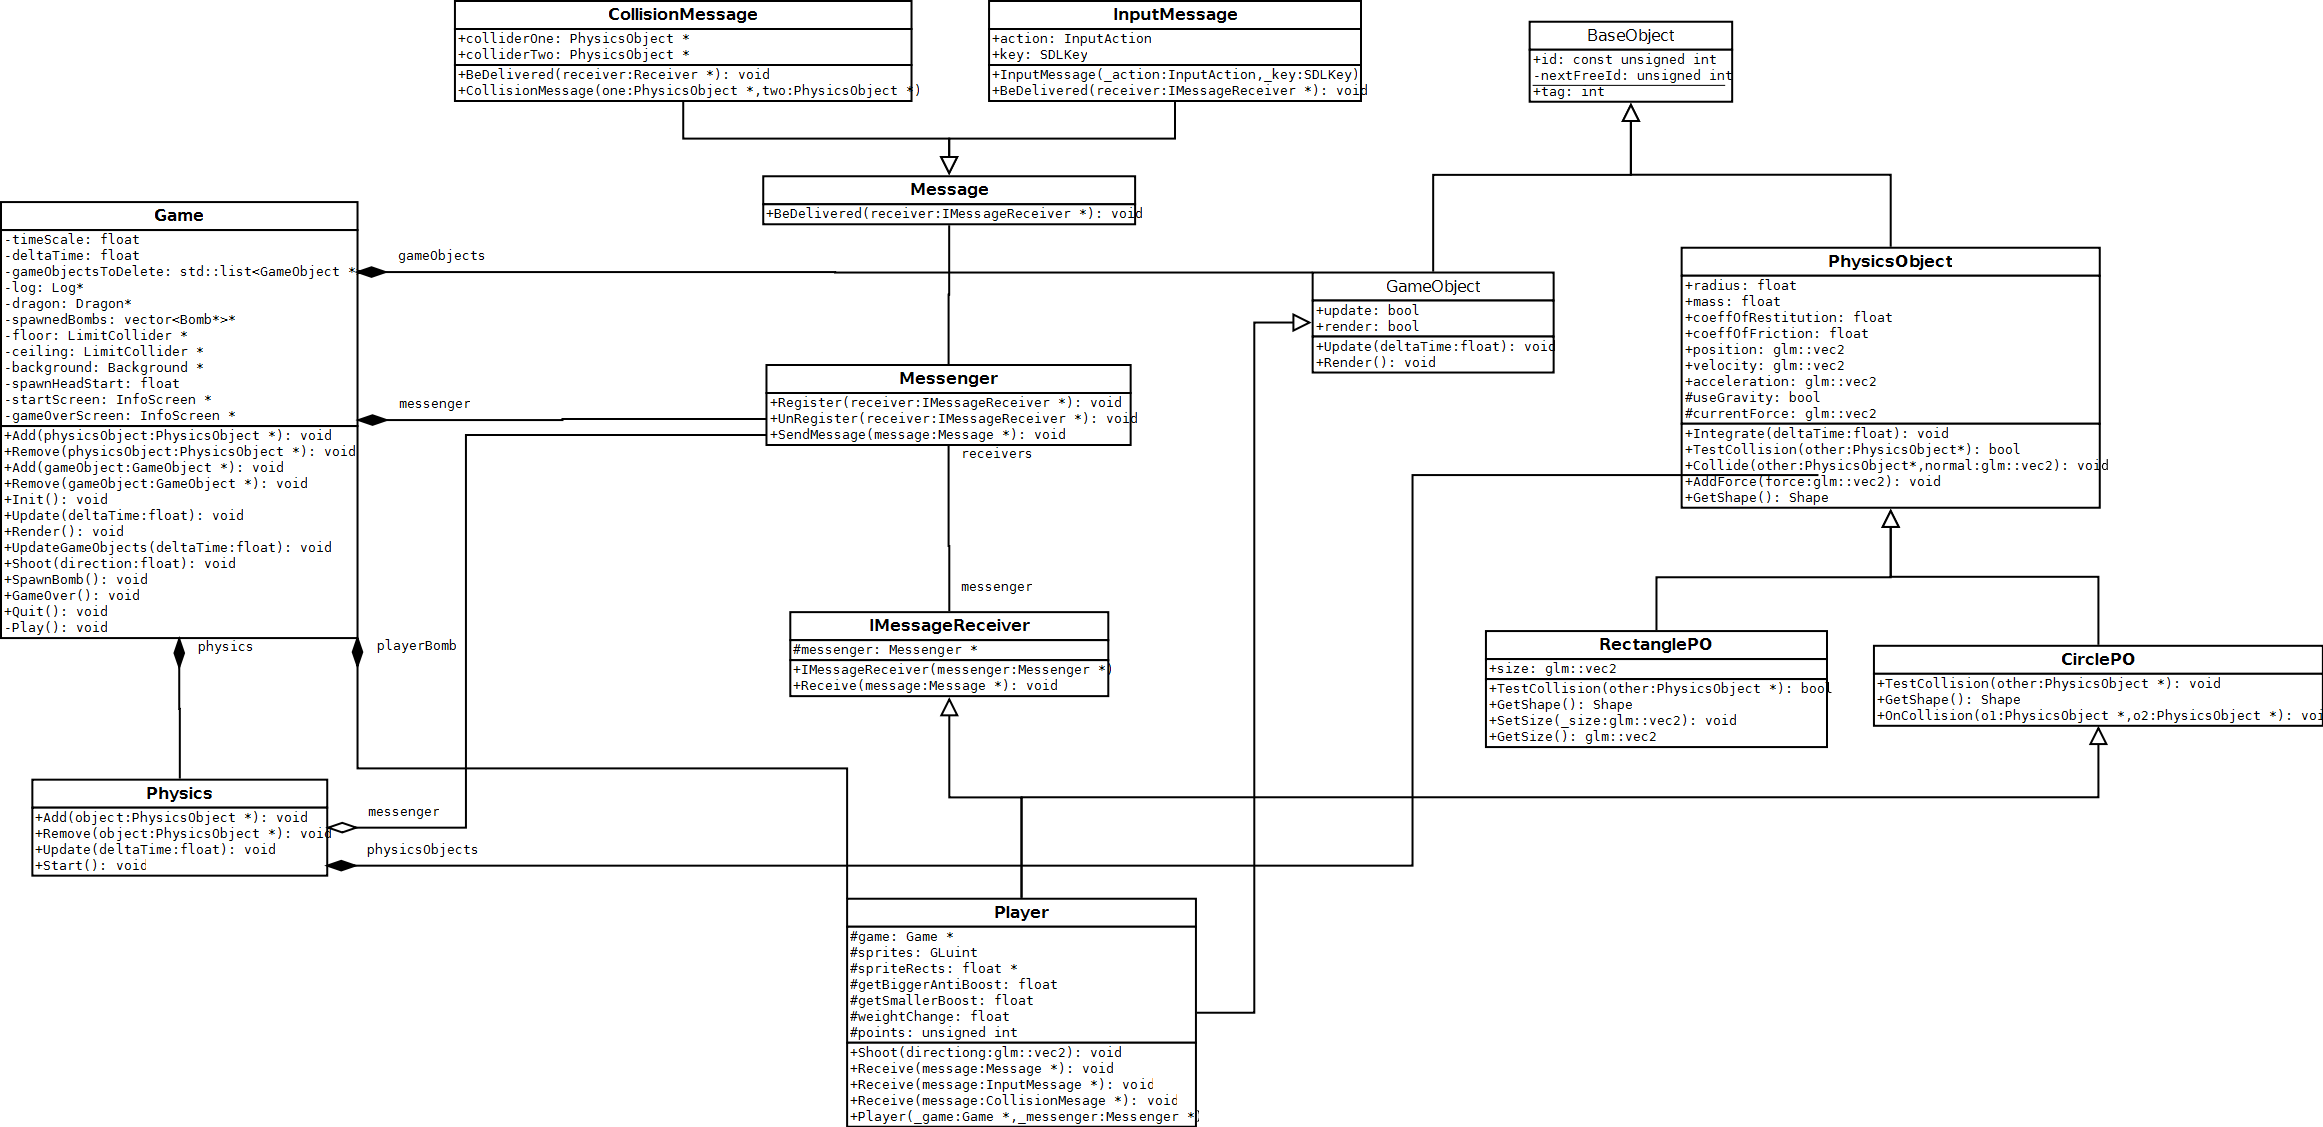
\includegraphics[totalheight=0.45\textheight, angle=90]{classes.png}
	\caption{A sketch of the most important classes.}
	\label{figure:classes}
\end{figure}

%-----------------------------------------
\section{Workflow}
\label{section:workflow}

I started working on the project quite early, because I wanted to try new things. So I tried and tried and jumped from one interesting thing to the next. I tried many graphics frameworks (openFrameworks, SDL, openGL, freeImage) I wanted to further my openGL skills, so I set up openGL (as well as the other frameworks). I decided to use openGL. So I created the drawing context and used the openGL display/event callbacks. (Which was a mistake, since the assignment was to create the loop and event system ourselves, but I only realized that later.) I got that running, so I created the physics logic (which I mostly reused in the final project). After that, however, things became chaotic. There were many loose ends which would have to be tied to the rest of the project. I would not have enough time to do that AND finish the other projects. Two weeks ago I decided to let it rest in peace. (It rests on GitHub: \url{https://github.com/JungleJinn/GE---Physics-Engine})

I took the good stuff and used it for a new, clean, and simple project, which is the one described in this report. I had a better vision of what I wanted to do from the beginning. It worked better. Even if it is only a small and simple thing, I hope the work it took to get to this point is visible.

\newpage
\lstlistoflistings
\listoffigures

\end{document}